\documentclass[twocolumn,aps,prb,10pt,amsmath,amssymb,amsthm,superscriptaddress]{revtex4-2}

\usepackage{newtxtext}
\usepackage{newtxmath}
\usepackage{microtype}

\usepackage{graphicx}
\usepackage{dcolumn}
\usepackage{bm}
\usepackage{multirow}
\usepackage{xcolor}
\usepackage{braket}
\usepackage{CJK}
\usepackage{indentfirst}
\usepackage{cases}

\usepackage{mathtools}

\def\Eq#1{Eq.~(\ref{#1})}
\def\Fig#1{Fig.~\ref{#1}}
\def\avg#1{\left\langle#1\right\rangle}
\newcommand{\cn}[1]{\begin{CJK*}{UTF8}{gbsn}#1\end{CJK*}}
\newcommand{\ZXL}[1]{{\bf \color{blue}ZXL: }{\color{red} #1}}
\newcommand{\bea}{\begin{eqnarray}}
\newcommand{\eea}{\end{eqnarray}}

\newcommand{\Tr}{\operatorname{Tr}}
\newcommand{\diag}{\operatorname{diag}}
\newcommand{\dd}{\mathrm{d}}
\newcommand{\ee}{\mathrm{e}}
\newcommand{\ii}{\mathrm{i}}
\newcommand{\trans}{\mathsf{T}}
\newcommand{\hc}{\dagger}
\newcommand{\mc}[1]{\mathcal{#1}}
\newcommand{\bb}[1]{\bm{#1}}

\newtheorem{theorem}{Theorem}
\newtheorem{lemma}{Lemma}
\newtheorem{proposition}{Proposition}
\newtheorem{corollary}{Corollary}
\theoremstyle{remark}
\newtheorem{remark}{Remark}

\usepackage[
    colorlinks,
    citecolor=blue,
    linkcolor=blue,
    urlcolor=blue,
]{hyperref}
\newcommand{\subref}[1]{\textcolor{blue}{#1}}
\newcommand{\ror}[2]{\href{https://ror.org/#1}{#2}}

\usepackage{orcidlink}
\usepackage{lipsum}

\begin{document}

\title{Sign-problem-free Bosonic Auxiliary Field Quantum Monte Carlo}

\author{Yin-Kai Yu\,\orcidlink{0009-0006-2589-2772}}
\affiliation{Beijing National Laboratory for Condensed Matter Physics\\ \& \ror{05cvf7v30}{Institute of Physics, Chinese Academy of Sciences}, Beijing 100190, China}
\affiliation{\ror{05qbk4x57}{University of Chinese Academy of Sciences}, Beijing 100049, China}

\author{Zhong-Chao Wei\,\orcidlink{0000-0002-1708-4306}}
\email{zcwei@thp.uni-koeln.de}
\affiliation{Qingdao Binhai University, Qingdao 266555, China}

\author{Lei Wang\,\orcidlink{0009-0004-1348-8583}}
\email{wanglei@iphy.ac.cn}
\affiliation{Beijing National Laboratory for Condensed Matter Physics\\ \& \ror{05cvf7v30}{Institute of Physics, Chinese Academy of Sciences}, Beijing 100190, China}
\affiliation{\ror{05qbk4x57}{University of Chinese Academy of Sciences}, Beijing 100049, China}
\affiliation{\ror{020vtf184}{Songshan Lake Materials Laboratory}, Dongguan, Guangdong 523808, China}

\author{Zi-Xiang Li\,\orcidlink{0000-0002-3941-365X}}
\email{zixiangli@iphy.ac.cn}
\affiliation{Beijing National Laboratory for Condensed Matter Physics\\ \& \ror{05cvf7v30}{Institute of Physics, Chinese Academy of Sciences}, Beijing 100190, China}
\affiliation{\ror{05qbk4x57}{University of Chinese Academy of Sciences}, Beijing 100049, China}

\date{\today}

\begin{abstract}
    Auxiliary-field quantum Monte Carlo (AFQMC) is one of the most powerful unbiased approaches to interacting quantum matter, but a systematic sign-problem-free formulation for bosons has long been missing. In this work we formulate finite-temperature bosonic AFQMC (BAFQMC) for generic interacting bosonic Hamiltonians, including decouplings that generate anomalous pairing terms at the one-body level. We derive the bosonic Gaussian trace formula, the equal-time Green's function, and exact local-update ratios in a notation tailored to Monte Carlo sampling. We then identify two symmetry routes to nonnegative configuration weights: reflection positivity and time-reversal symmetry. These results show that, unlike in world-line formulations, geometric frustration does not by itself forbid sign-problem-free bosonic simulations once the problem is rewritten in auxiliary-field language, thereby opening a new exact-simulation territory beyond world-line QMC and stochastic series expansion. We further present explicit sign-problem-free model classes and proof-of-principle benchmarks on frustrated two-flavor Bose-Hubbard models on the triangular lattice, for both number-conserving and paired formulations, where BAFQMC agrees with exact diagonalization. Finally, we discuss the pole structure of the bosonic sampling weights and the practical regime of applicability of the present finite-temperature algorithm.
\end{abstract}

\maketitle

\section{Introduction}

Quantum Monte Carlo (QMC) methods provide some of the most reliable nonperturbative tools for correlated quantum matter. Their basic idea is to rewrite the partition function as a sum or integral over a large configuration space and then evaluate that statistical ensemble by importance sampling. When the sampled weights are nonnegative, the resulting algorithms are often polynomial in system size and inverse temperature and can deliver numerically exact thermodynamic observables with controlled systematic errors. The fundamental obstacle is the sign problem: once the statistical weight fluctuates in sign or phase, the signal-to-noise ratio decays exponentially with system size or inverse temperature. In practice, the boundary between sign-free and sign-problematic formulations is one of the sharpest boundaries between tractable and intractable strongly correlated models.

For bosonic and spin systems, the standard intuition about that boundary comes from local-weight formulations such as world-line QMC and stochastic series expansion (SSE). In those approaches, frustration in the off-diagonal matrix elements of the Hamiltonian is a primary source of negative weights. On bipartite or otherwise unfrustrated lattices, a Marshall sign transformation or a suitable basis choice can often make all local amplitudes nonnegative; on geometrically frustrated lattices, the same strategy usually fails. This consensus regarding the sign problem in bosonic QMC is useful, but it is also tied to algorithms that sample local paths or operator strings. It does not decide the sign structure once the microscopic bosons are traced out analytically before Monte Carlo sampling.

Auxiliary-field quantum Monte Carlo belongs precisely to that different class. In AFQMC one decouples the interaction with Hubbard-Stratonovich (HS) fields, integrates out the quantum operators exactly for each auxiliary-field configuration, and samples the resulting global weight. For fermions, this leads to determinantal weights and to a large body of work on sign-problem-free models. 
The key lesson from that literature is that positivity is controlled not by local matrix elements but by the symmetries of the decoupled one-body propagators. Within the fermionic AFQMC framework, it has been proven that sign-problem-free simulations are feasible if the decoupled Hamiltonian possesses reflection positivity (RP) or time-reversal symmetry (TRS) in either the fermion or Majorana fermion representations. Those ideas dramatically expanded the class of fermionic models accessible to unbiased simulation.

For bosons, however, an analogous framework has been missing. Bosonic auxiliary-field schemes have appeared previously, for example for Bose-Fermi mixtures and in canonical-ensemble formulations, but the bosonic sign structure has not been analyzed in a systematic and symmetry-based way. The technical obstacles are also different from the fermionic case. The trace of a bosonic Gaussian operator is subtler because the trace formula used for calculating Monte Carlo sampling weights exhibits a pole structure and does not converge naturally. At the same time, even when the trace formula is available, one still needs practical criteria that guarantee nonnegative Monte Carlo weights after HS decoupling. These issues have so far prevented a general sign-problem-free formulation of BAFQMC.

The main advance of this work is to close that gap. We formulate finite-temperature bosonic auxiliary-field quantum Monte Carlo, abbreviated below as BAFQMC, in a way that is directly suitable for sign-problem analysis, and we identify rigorous symmetry conditions under which the configuration weights are nonnegative. This is not a minor extension of existing bosonic QMC technology. Rather, it shows that the sign-free region for bosonic systems is substantially larger in auxiliary-field language than in local-weight language. In particular, frustrated bosonic models that remain inaccessible to world-line QMC or SSE can become sign-problem-free in BAFQMC when the HS-decoupled one-body propagators obey reflection positivity or time-reversal symmetry.

Our results have three layers. First, at the formal level, we derive the bosonic Gaussian trace formula, the equal-time Green's function, and exact local-update ratios for generic finite-temperature BAFQMC, allowing both number-conserving and paired one-body propagators. Second, at the conceptual level, we establish two sign-free mechanisms. One is a bosonic reflection-positivity criterion formulated directly at the operator level. The other is a time-reversal-symmetry criterion for number-conserving decouplings, where the time-reversal operator is a Kramers antiunitary symmetry with $\Theta^2=-1$. Third, at the practical level, we give explicit model classes that satisfy these criteria and present proof-of-principle benchmarks on frustrated two-flavor Bose-Hubbard models on the triangular lattice, for both number-conserving and paired formulations, where sign-free BAFQMC agrees with exact diagonalization.

These results are summarized schematically in Fig.~\ref{fig:schematic}. For unfrustrated bosonic models, local-weight methods such as SSE and world-line QMC remain excellent and often simplest choices. BAFQMC does something qualitatively different: it opens a sign-free route into the frustrated sector, provided that reflection positivity (RP) or time-reversal symmetry (TRS) is present in the HS-decoupled problem. The upper-left quadrant of Fig.~\ref{fig:schematic}, characterized by frustration together with RP/TRS, is therefore the new computable territory unlocked by this work.

The rest of the paper is organized as follows. Section~\ref{sec:afqmc} formulates BAFQMC and derives the basic weight and Green-function formulas. Section~\ref{sec:positive} establishes the reflection-positivity and time-reversal-symmetry criteria for nonnegative weights. Section~\ref{sec:examples} presents explicit sign-problem-free models and minimal benchmark results. Section~\ref{sec:discussion} discusses the significance of the method together with the pole structure and practical limitations of the finite-temperature sampling weights. We summarize and outline future directions in Sec.~\ref{sec:summary}. Technical derivations, including the algebra of bosonic quadratic forms, the Gaussian trace formula, the update ratio, and the regularized interpretation of the weight, are collected in the appendices.

\begin{figure}[bt]
    \centering
    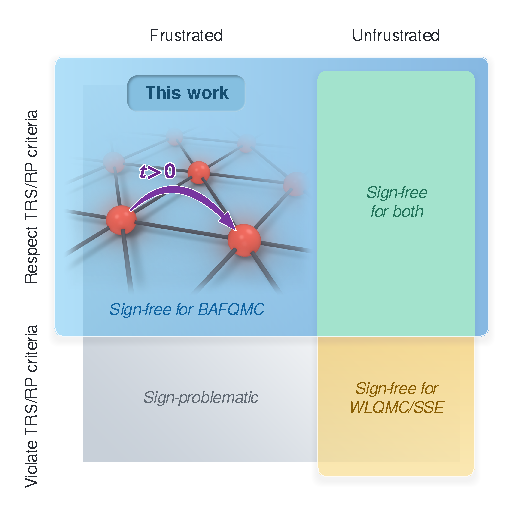
\includegraphics[width=\linewidth]{figures/schematic.pdf}
    \caption{\textbf{Schematic classification of the sign problem in bosonic systems.} The diagram divides systems into four quadrants based on the presence of reflection positivity (RP) or time-reversal symmetry (TRS), and the presence of lattice frustration. For bosonic systems possessing RP or TRS, BAFQMC is sign-free, corresponding to the upper half-plane (highlighted in blue) in the schematic diagram. For systems without lattice frustration, Stochastic Series Expansion (SSE) and World-line QMC (WLQMC) are sign-free, corresponding to the right half-plane (highlighted in yellow) of the schematic diagram. Among these, the upper-left region characterized by frustration but possessing RP or TRS represents the new computable territory revealed by this work.}
    \label{fig:schematic}
\end{figure}




\section{AFQMC for bosonic systems}
\label{sec:afqmc}

\subsection{Quadratic bosonic generators and Hubbard-Stratonovich decoupling}

We consider a system of $N$ bosonic modes collected into the column vector
\begin{equation}
    \hat{\bb a} = (\hat a_1,\ldots,\hat a_N)^\trans,
\end{equation}
and define the Nambu spinor
\begin{equation}
    \hat\chi = (\hat{\bb a},\hat{\bb a}^{\hc})^\trans.
\end{equation}
Its canonical commutation relations are encoded by the symplectic form
\begin{equation}
    [\hat\chi_\mu,\hat\chi_\nu] = \Omega_{\mu\nu},
    \qquad
    \Omega =
    \begin{pmatrix}
        0 & I_N \\
        -I_N & 0
    \end{pmatrix}.
\end{equation}
A general one-body bosonic operator can be written as
\begin{equation}
    \hat h(A,\xi) = -\frac12 \hat\chi^\trans \Omega A \hat\chi + \xi,
    \label{eq:hAdef}
\end{equation}
where $A$ belongs to the complex symplectic Lie algebra,
\begin{equation}
    \Omega A + A^\trans \Omega = 0,
    \label{eq:symplectic_condition}
\end{equation}
and $\xi\in\mathbb C$ is a scalar shift. In block form,
\begin{equation}
    A =
    \begin{pmatrix}
        K & \Delta \\
        -\overline{\Delta} & -K^\trans
    \end{pmatrix},
    \qquad
    \Delta^\trans = \Delta,
\end{equation}
which gives
\begin{equation}
\begin{aligned}
    \hat h(A,\xi)
    ={}& \hat{\bb a}^{\hc} K\hat{\bb a}
    + \frac12\hat{\bb a}^{\hc}\Delta\hat{\bb a}^{\hc\trans}
    + \frac12\hat{\bb a}^\trans\overline{\Delta}\hat{\bb a} \\
    &\quad + \xi + \frac12\Tr K.
\end{aligned}
\label{eq:block_form_h}
\end{equation}
The scalar $\xi$ is essential: it absorbs the normal-ordering constant $\frac12\Tr K$ and allows us to represent physical quadratic Hamiltonians without ambiguity.

We study interacting bosonic Hamiltonians of the form
\begin{equation}
    \hat H = \hat H_0 + \hat H_{\mathrm{int}},
\end{equation}
with $\hat H_0$ a one-body operator and $\hat H_{\mathrm{int}}$ an interaction that can be decomposed into squares of one-body operators,
\begin{equation}
    \hat H_{\mathrm{int}} = \sum_\gamma \lambda_\gamma \hat O_\gamma^2.
    \label{eq:hint_square}
\end{equation}
This includes the standard Bose-Hubbard density interaction, density-density interactions between different sites or flavors, and many spin interactions once written in a bosonic representation. A Trotter-Suzuki decomposition at inverse temperature $\beta=L_\tau\Delta\tau$ gives
\begin{equation}
    Z = \Tr\,\ee^{-\beta \hat H}
    = \Tr\left[\prod_{\ell=1}^{L_\tau} \ee^{-\Delta\tau \hat H_0}\ee^{-\Delta\tau \hat H_{\mathrm{int}}}\right]
    + O(\Delta\tau^2).
\end{equation}
For each interaction channel we may apply a continuous HS transformation,
\begin{equation}
    \ee^{-\Delta\tau \lambda_\gamma \hat O_\gamma^2}
    = \int \dd\phi_\gamma\, p_\gamma(\phi_\gamma)
    \ee^{s_\gamma \phi_\gamma \hat O_\gamma},
    \qquad
    s_\gamma^2 = -2\Delta\tau\lambda_\gamma,
    \label{eq:hs_generic}
\end{equation}
where the contour and the Gaussian factor $p_\gamma$ depend on the sign of $\lambda_\gamma$. For attractive channels one may take $s_\gamma\in\mathbb R$ and integrate over real fields; for repulsive channels one may equivalently use imaginary shifts or discrete decompositions. Nothing in the formalism below depends on the specific HS choice, provided that after decoupling every time-slice propagator is Gaussian.

Introducing all auxiliary fields collectively as $\phi$, the partition function takes the AFQMC form
\begin{equation}
    Z = \int \mc D\phi\; P_{\mathrm{aux}}(\phi)\, W(\phi),
    \label{eq:Z_afqmc}
\end{equation}
where $P_{\mathrm{aux}}(\phi)$ is the product of bare HS measures and
\begin{equation}
    W(\phi) = \Tr\, \hat U(\phi),
    \qquad
    \hat U(\phi) = \prod_{\ell=1}^{L} \ee^{\hat h_\ell(\phi_\ell)}.
    \label{eq:weight_def}
\end{equation}
Here $L$ denotes the total number of Gaussian factors after Trotter splitting and HS decoupling, and each
\begin{equation}
    \hat h_\ell(\phi_\ell) = \hat h\left(A_\ell(\phi_\ell),\xi_\ell(\phi_\ell)\right)
\end{equation}
is a bosonic quadratic generator of the form in Eq.~\eqref{eq:hAdef}. The bosonic sign problem is the statement that $W(\phi)$ cannot be chosen real and nonnegative for all auxiliary-field configurations. The remainder of this section derives the explicit Gaussian formula for $W(\phi)$ and the observables needed in a Monte Carlo implementation.

\subsection{Bosonic Gaussian trace formula}

The fundamental algebraic fact is that a bosonic Gaussian propagator acts linearly on the Nambu operators. As shown in Appendix~\ref{app:algebra},
\begin{equation}
    [\hat h(A,\xi),\hat\chi] = -A\hat\chi,
    \label{eq:commutator_key}
\end{equation}
so that
\begin{equation}
    \ee^{\hat h(A,\xi)}\hat\chi\,\ee^{-\hat h(A,\xi)} = \ee^{-A}\hat\chi,
    \qquad
    \hat\chi\,\ee^{\hat h(A,\xi)} = \ee^{\hat h(A,\xi)}\ee^{A}\hat\chi.
    \label{eq:linear_action}
\end{equation}
For the full ordered product \eqref{eq:weight_def}, we therefore have
\begin{equation}
    \hat\chi\,\hat U(\phi) = \hat U(\phi)\,\mc M(\phi)\hat\chi,
    \qquad
    \mc M(\phi) = \ee^{A_1}\ee^{A_2}\cdots \ee^{A_L}.
    \label{eq:Mdef}
\end{equation}
The matrix $\mc M$ is the single-particle transfer matrix associated with the auxiliary-field configuration.

Whenever the ordinary bosonic trace exists, the weight is given by the bosonic Gaussian trace formula
\begin{equation}
    W(\phi) = \exp\!\left[\sum_{\ell=1}^L \xi_\ell(\phi_\ell)\right]
    \det\!\left(I_{2N}-\mc M\left(\phi\right)\right)^{-1/2}.
    \label{eq:trace_formula_main}
\end{equation}
The square root is the metaplectic branch, fixed by continuity from a stable reference region where the trace is manifestly convergent; Appendix~\ref{app:trace} explains this point in detail and derives the formula in a way that makes the branch choice explicit. Equation~\eqref{eq:trace_formula_main} is the bosonic analogue of the familiar fermionic determinantal weight, with two important differences. First, bosonic convergence is not automatic; second, anomalous terms lead naturally to a square root rather than to an ordinary determinant.

The number-conserving case is simpler and deserves separate emphasis. If every slice contains no pairing term, then we may write
\begin{equation}
    \hat h_\ell = \hat{\bb a}^{\hc} B_\ell \hat{\bb a} + \xi_\ell,
    \label{eq:number_conserving_slice}
\end{equation}
with an $N\times N$ matrix $B_\ell$, and the corresponding single-particle product is
\begin{equation}
    \mc B = \ee^{B_1}\ee^{B_2}\cdots\ee^{B_L}.
\end{equation}
Then the bosonic weight is single-valued and takes the familiar form
\begin{equation}
    W(\phi)=\exp\!\left[\sum_{\ell=1}^L \xi_\ell(\phi_\ell)\right]
    \det\!\left(I_N-\mc B(\phi)\right)^{-1}.
    \label{eq:trace_formula_number}
\end{equation}
This formula is derived directly in Appendix~\ref{app:trace_number} using coherent states. It reduces the bosonic sampling problem to the analysis of an ordinary determinant and is the natural starting point for the time-reversal-symmetry criterion of Sec.~\ref{sec:trs}.

In physically stable regimes the ordinary trace and the determinant expressions above coincide. Outside those regimes one must distinguish two situations. For paired evolutions, such as the reflection-positive paired model of Eq.~\eqref{eq:benchmark_pairing}, the sampled configurations relevant in practice stay inside a connected component of $\det(I_{2N}-\mc M)\neq 0$; the metaplectic formula is then fixed by continuity from the convergent region. The number-conserving case is subtler. Because the auxiliary-field integral can cross $\det(I_N-\mc B)=0$, a configuration-by-configuration analytic continuation is no longer the right interpretation of the Monte Carlo weight. There one should instead read Eq.~\eqref{eq:trace_formula_number} as the renormalized finite part selected by a Gaussian cutoff in occupation-number space, as explained in Appendix~\ref{app:regularization}.





\subsection{Equal-time Green's function and observables}

At fixed auxiliary field, all equal-time observables follow from the bosonic Green's function
\begin{equation}
    G(\phi)_{\mu\nu}
    = \frac{\Tr\left[\hat\chi_\mu\hat\chi_\nu\hat U(\phi)\right]}{\Tr\,\hat U(\phi)}.
    \label{eq:Gdef}
\end{equation}
Using Eq.~\eqref{eq:Mdef} and cyclicity of the trace, Appendix~\ref{app:green} shows that
\begin{equation}
    G(\phi) = \left(I_{2N}-\mc M(\phi)\right)^{-1}\Omega.
    \label{eq:Gformula}
\end{equation}
This compact expression is the bosonic counterpart of the equal-time Green's function in fermionic AFQMC. Since $\Omega^{-1}=-\Omega$, one also has
\begin{equation}
    G(\phi)\Omega^{-1} = \left(I_{2N}-\mc M(\phi)\right)^{-1}.
    \label{eq:Gomega_inverse}
\end{equation}
The four $N\times N$ blocks of $G$ give, respectively, the anomalous correlators $\langle \hat a_i\hat a_j\rangle_\phi$, the normal correlators $\langle \hat a_i\hat a_j^\hc\rangle_\phi$, $\langle \hat a_i^\hc\hat a_j\rangle_\phi$, and $\langle \hat a_i^\hc\hat a_j^\hc\rangle_\phi$.

In the number-conserving case Eq.~\eqref{eq:Gformula} reduces to the more familiar matrix identities
\begin{equation}
    \langle \hat a_i \hat a_j^\hc\rangle_\phi = \left(I_N-\mc B\right)^{-1}_{ij},
    \qquad
    \langle \hat a_j^\hc \hat a_i\rangle_\phi = \left[\mc B\left(I_N-\mc B\right)^{-1}\right]_{ij}.
    \label{eq:number_green_blocks}
\end{equation}
All higher-order equal-time correlators follow from Wick's theorem because $\hat U(\phi)$ is a Gaussian operator. Thus, once the matrix $G(\phi)$ is known, one may evaluate arbitrary local observables, structure factors, and susceptibilities by standard Gaussian contraction rules.

\subsection{Importance sampling and local updates}

The Monte Carlo weight for an auxiliary-field configuration is
\begin{equation}
    P(\phi) = P_{\mathrm{aux}}(\phi)\,W(\phi).
\end{equation}
For a local proposal that changes a single auxiliary field from $\phi$ to $\phi'$, the Metropolis acceptance probability is
\begin{equation}
    p_{\mathrm{acc}}(\phi\to\phi') =
    \min\!\left\{1,
    \frac{P_{\mathrm{aux}}(\phi')}{P_{\mathrm{aux}}(\phi)}
    \frac{W(\phi')}{W(\phi)}\right\}.
\end{equation}
Suppose only slice $\ell$ is modified, with
\begin{equation}
    \ee^{A_\ell'} = \left(I_{2N}+\Delta_\ell\right)\ee^{A_\ell},
    \qquad
    \delta\xi_\ell = \xi_\ell' - \xi_\ell.
    \label{eq:delta_def}
\end{equation}
Note that the $\delta\xi_\ell$ here originates from the commutator term when the Hamiltonian is written in the Nambu representation.
Introduce the cyclically ordered product starting at slice $\ell$,
\begin{equation}
    \mc M_\ell = \ee^{A_\ell}\ee^{A_{\ell+1}}\cdots \ee^{A_L}\ee^{A_1}\cdots \ee^{A_{\ell-1}},
\end{equation}
and its corresponding Green's function
\begin{equation}
    G_\ell = \left(I_{2N}-\mc M_\ell\right)^{-1}\Omega.
\end{equation}
Then Appendix~\ref{app:update} shows that the exact Gaussian weight ratio is
\begin{equation}
    \frac{W(\phi')}{W(\phi)}
    = \ee^{\delta\xi_\ell}
    \det\!\left[I_{2N}+\Delta_\ell\left(I_{2N}-G_\ell\Omega^{-1}\right)\right]^{-1/2}.
    \label{eq:update_ratio_main}
\end{equation}
This is the bosonic analogue of the fast-update determinant ratio in determinantal QMC. When the local modification affects only a few matrix elements, the matrix inside the determinant differs from the identity by a low-rank operator and can be evaluated using a reduced determinant.

At low temperatures or long imaginary time, the matrix products $\mc M$ and $\mc B$ become strongly ill-conditioned. This numerical issue is familiar from fermionic AFQMC and must also be handled here by stabilized matrix decompositions. In the number-conserving case, standard QR or SVD stabilization applies directly to the product $\mc B$. In the paired case, one may use structure-preserving factorizations for symplectic products. Since the present paper focuses on the sign structure rather than on implementation details, we do not expand on stabilization algorithms further, but we emphasize that the positivity results of Sec.~\ref{sec:positive} are independent of the particular stabilization scheme used in practice.






    
\section{Conditions for nonnegative weights}
\label{sec:positive}

We now turn to the main conceptual question: under what conditions is the BAFQMC weight nonnegative for every auxiliary-field configuration? In contrast to world-line methods, the answer is not controlled by local signs of matrix elements. Instead, it is determined by the algebraic structure of the Gaussian propagators generated after HS decoupling. We focus on two symmetry mechanisms. Reflection positivity works directly at the operator level and naturally allows pairing terms. Time-reversal symmetry, in the sense of a Kramers antiunitary symmetry with $\Theta^2=-1$, gives a particularly transparent determinant criterion in the number-conserving case.

\subsection{Reflection positivity}
\label{sec:reflection}

The concept of reflection positivity was originally introduced in the context of axiomatic quantum field theory~\cite{osterwalder1973axioms}. It has since become a standard mathematical tool in statistical physics~\cite{kondratiev2006reflection,biskup2009reflection}. Its main application in strongly correlated systems started from Lieb's work on spin reflection positivity in the Hubbard model~\cite{lieb1989prl}. Majorana reflection positivity was then proposed~\cite{jaffe2015reflection,jaffe2016characterization} and applied to interacting spinless fermion models~\cite{wei2015prb}. The connection between Majorana reflection positivity and sign-problem-free quantum lattice fermion models was subsequently clarified in Ref.~\cite{wei2016prl}. The bosonic case considered here is simpler in one important respect: the reflected left and right algebras commute rather than anticommute.

Let $\mc F_L$ and $\mc F_R$ be two bosonic Fock spaces generated by annihilation operators $\hat b_i$ and $\hat c_i$ ($i=1,\dots,M$), and let the full Hilbert space be $\mc F=\mc F_L\otimes \mc F_R$. We denote by $\mathfrak A_L$ the algebra generated by $\hat b_i$ and $\hat b_i^\hc$, and by $\mathfrak A_R$ the algebra generated by $\hat c_i$ and $\hat c_i^\hc$. Define an antilinear reflection map $\theta:\mathfrak A_L\to\mathfrak A_R$ through
\begin{equation}
    \theta(\ii) = -\ii,
    \qquad
    \theta(\hat b_i)=\hat c_i,
    \qquad
    \theta(\hat b_i^\hc)=\hat c_i^\hc,
    \label{eq:theta_def}
\end{equation}
and extend it multiplicatively. The reflection need not coincide with a literal spatial reflection. Any decomposition into two commuting and isomorphic bosonic algebras works equally well.

A natural reflection-positive cone is
\begin{equation}
    \mc K_\theta = \left\{\sum_r \hat R_r\,\theta(\hat R_r)\;;\; \hat R_r\in\mathfrak A_L\right\}.
    \label{eq:cone_def}
\end{equation}
Two elementary facts are enough for our purposes. First, $\mc K_\theta$ is closed under addition and multiplication. Addition is obvious from the definition. For multiplication, one uses only that every operator in $\mathfrak A_L$ commutes with every operator in $\mathfrak A_R$:
\begin{equation}
    \hat R\theta(\hat R)\,\hat S\theta(\hat S)
    = \hat R\hat S\,\theta(\hat R\hat S),
\end{equation}
which is again in $\mc K_\theta$. Second, whenever the trace exists, every $\hat X\in\mc K_\theta$ has nonnegative trace. Indeed, for a single term $\hat R\theta(\hat R)$, the factorized Hilbert space gives
\begin{equation}
    \Tr_{\mc F}\!\left[\hat R\theta(\hat R)\right]
    = \Tr_{\mc F_L}(\hat R)\,\Tr_{\mc F_R}(\theta(\hat R))
    = \left|\Tr_{\mc F_L}(\hat R)\right|^2 \ge 0,
\end{equation}
where in the last step one chooses identical occupation-number bases on the two Fock spaces and uses the antilinearity of $\theta$. Summing over terms then gives $\Tr\,\hat X\ge 0$ for every $\hat X\in \mc K_\theta$.

This immediately leads to a sign-free criterion for BAFQMC. If every slice propagator satisfies
\begin{equation}
    \ee^{\hat h_\ell(\phi_\ell)} \in \ee^{\xi_\ell(\phi_\ell)}\mc K_\theta,
    \qquad
    \xi_\ell(\phi_\ell)\in\mathbb R,
    \label{eq:rp_slice_condition}
\end{equation}
then the full ordered product also lies in $\ee^{\sum_\ell \xi_\ell(\phi_\ell)}\mc K_\theta$ because $\mc K_\theta$ is multiplicatively closed, and therefore
\begin{equation}
    W(\phi)=\Tr\prod_{\ell=1}^{L}\ee^{\hat h_\ell(\phi_\ell)}\ge 0.
    \label{eq:rp_weight_nonnegative}
\end{equation}

A convenient operator-level sufficient condition is the following. Suppose a slice generator can be written as
\begin{equation}
    \hat h = \hat q + \theta(\hat q) + \sum_{\mu,\nu=1}^{m} K_{\mu\nu}\,\hat X_\mu\,\theta(\hat X_\nu) + \xi,
    \label{eq:rp_generator}
\end{equation}
where $\hat q,\hat X_\mu\in\mathfrak A_L$, $K=K^\hc\succeq 0$, and $\xi\in\mathbb R$. Then $\ee^{\hat h}\in \ee^{\xi}\mc K_\theta$. The reason is simple. Because left and right operators commute,
\begin{equation}
    \ee^{\hat q+\theta(\hat q)} = \ee^{\hat q}\theta(\ee^{\hat q}) \in \mc K_\theta.
\end{equation}
For the mixed term, positivity of $K$ allows us to write $K=R^\hc R$ and define $\hat Y_a=\sum_\mu R_{a\mu}\hat X_\mu$, so that
\begin{equation}
    \sum_{\mu,\nu}K_{\mu\nu}\hat X_\mu\theta(\hat X_\nu)
    = \sum_a \hat Y_a\theta(\hat Y_a).
\end{equation}
Then the exponential $\ee^{\hat Y_a\theta(\hat Y_a)}$ is a series of reflected squares and therefore belongs to $\mc K_\theta$ term by term. A standard Lie-Trotter product formula~\cite{trotter1959product} then shows that the full exponential $\ee^{\hat h}$ also belongs to the positive cone $\mc K_\theta$.

For Gaussian bosonic slices, the practically useful specialization of Eq.~\ref{eq:rp_generator} is obtained by taking $\hat q$ quadratic in the left bosons and $\hat X_\mu$ linear in them. 
In the Nambu basis
\begin{equation}
    \hat\chi = (\hat{\bb b},\hat{\bb b}^{\hc},\hat{\bb c},\hat{\bb c}^{\hc})^\trans,
\end{equation}
a generic reflection-positive Gaussian slice takes the form
\begin{equation}
    \hat h = \hat\chi^\trans
    \begin{pmatrix}
        D & F \\
        F^\trans & \bar D
    \end{pmatrix}
    \hat\chi + \xi,
    \qquad F = F^\hc \succeq 0.
    \label{eq:rp_block_form}
\end{equation}
This criterion allows arbitrary quadratic terms $D$ within each reflected half and arbitrary positive semidefinite couplings $F$ between the two halves. In particular, it naturally compatible with geometrically frustrated lattices. From a practical Monte Carlo viewpoint, Eq.~\eqref{eq:rp_block_form} is a convenient RP test: once each HS-decoupled slice can be written in this form, every slice belongs to the RP cone and the configuration weight is nonnegative. In Sec.~\ref{sec:models} we will use exactly this viewpoint to identify sign-problem-free number-conserving and paired models on the triangular lattice.

One more comment is needed because bosonic weights have poles. The cone argument above is literal whenever the bare trace converges absolutely. In actual BAFQMC, however, some configurations may lie outside that domain, so the weight has to be regularized. In paired RP models, including the benchmark of Eq.~\eqref{eq:benchmark_pairing}, the sampled trajectory stays inside a pole-free connected component, and the metaplectic weight is fixed by continuity from the convergent region. In number-conserving problems the auxiliary-field integral may instead cross $\det(I_N-\mc B)=0$, so a configuration-wise continuation is no longer adequate; Appendix~\ref{app:regularization} then defines the weight by Gaussian-cutoff renormalization.

The same RP condition can also be reformulated at the single-particle level in the semigroup language~\cite{wei2024prb}. There the Gaussian generator splits into a metric-preserving part and a cone part. For regularized sampling weights, the cone part of Gaussian generator can be decomposed into a direct sum of an element in a contraction semigroup and an element in an expansion semigroup. This semigroup picture is what guarantees that, in the paired RP sector where no singularity is crossed, the regularized Gaussian weight stays on the same nonnegative branch as the convergent bare trace. The details are given in Appendix~\ref{app:regularized_rp}.

\subsection{Time-reversal symmetry}
\label{sec:trs}

A second route to nonnegative weights arises when the decoupled propagators conserve boson number and possess time-reversal symmetry. Here time-reversal symmetry means a Kramers antiunitary symmetry $\Theta=UK$ on the single-particle space with $\Theta^2=-1$, or equivalently
\begin{equation}
    U U^* = -I_N,
    \label{eq:kramers_condition}
\end{equation}
where $K$ denotes complex conjugation and $U$ is unitary. For the two-flavor basis used below, a convenient phase convention is
\begin{equation}
    \Theta\hat b_i\Theta^{-1} = \hat c_i,
    \qquad
    \Theta\hat c_i\Theta^{-1} = -\hat b_i,
    \qquad
    \Theta\ii\Theta^{-1} = -\ii \, .
    \label{eq:trs_action_operator}
\end{equation}
Consider slice generators of the form
\begin{equation}
    \hat h_\ell = \hat{\bb a}^{\hc} B_\ell \hat{\bb a} + \xi_\ell,
    \qquad
    \xi_\ell\in\mathbb R,
    \label{eq:antiunitary_slice}
\end{equation}
so that the weight is given by Eq.~\eqref{eq:trace_formula_number}. Assume that every slice matrix satisfies
\begin{equation}
    U^\hc \overline{B_\ell} U = B_\ell,
    \qquad \ell=1,\ldots,L.
    \label{eq:Bsymmetry}
\end{equation}
Then the BAFQMC weight is real and nonnegative whenever it is finite.

The argument is direct. Because complex conjugation commutes with the matrix exponential, Eq.~\eqref{eq:Bsymmetry} is preserved by exponentiation and multiplication, so the full single-particle propagator
\begin{equation}
    \mc B = \ee^{B_1}\cdots\ee^{B_L}
\end{equation}
obeys the same symmetry, $U^\hc\overline{\mc B}U=\mc B$. Therefore every nonreal eigenvalue $\lambda$ of $\mc B$ is accompanied by its complex conjugate $\lambda^*$. For a real eigenvalue $r$, the corresponding eigenspace---or, if $\mc B$ is not diagonalizable, the corresponding generalized eigenspace---is invariant under $\Theta$. Kramers reasoning then shows that states come in linearly independent pairs $v$ and $\Theta v$, because $\Theta^2=-1$ forbids $v$ from being proportional to $\Theta v$~\cite{sakurai2017modern}. Hence every real eigenvalue has even algebraic multiplicity. As a result,
\begin{equation}
    \det(I_N-\mc B)
    = \prod_{\lambda\notin\mathbb R} |1-\lambda|^2
      \prod_{r\in\mathbb R} (1-r)^{m_r}
    \ge 0,
    \label{eq:det_nonnegative}
\end{equation}
where $m_r$ is even for every real eigenvalue $r$. Since the scalar prefactor in Eq.~\eqref{eq:trace_formula_number} is also positive for real $\xi_\ell$, the full weight satisfies $W(\phi)\ge0$ whenever the determinant is finite.

For two-flavor bosons this criterion takes a particularly convenient form. Writing
\begin{equation}
    \hat{\bb a} = (\hat b_1,\ldots,\hat b_M,\hat c_1,\ldots,\hat c_M)^\trans
\end{equation}
and choosing
\begin{equation}
    U = \ii\sigma_y\otimes I_M =
    \begin{pmatrix}
        0 & I_M \\
        -I_M & 0
    \end{pmatrix},
\end{equation}
Eq.~\eqref{eq:Bsymmetry} is equivalent to the block structure
\begin{equation}
    \hat h_\ell =
    \hat{\bb a}^\dagger
    \begin{pmatrix}
        D_\ell & F_\ell \\
        -\overline{F_\ell} & \overline{D_\ell}
    \end{pmatrix}
    \hat{\bb a}
    + \xi_\ell \,,
    \label{eq:block_TRS}
\end{equation}
with $D_\ell$ and $F_\ell$ arbitrary complex $M\times M$ matrices. The criterion itself allows arbitrary complex $D_\ell$ and $F_\ell$; the special case $F_\ell=0$ is only a convenient subclass used in some explicit examples below. 

Several remarks help place the criterion in context. First, the condition is imposed on the HS-decoupled one-body propagators, not on the bare interacting Hamiltonian in a particular basis. A model may look sign-problematic microscopically and still admit a sign-free BAFQMC decoupling. Second, the condition $\Theta^2=-1$ is essential. If an antiunitary symmetry squares to $+1$, eigenvalues still come in conjugate pairs, but real eigenvalues need not have even multiplicity, so the determinant can change sign. Third, the present time-reversal-symmetry argument is restricted to number-conserving slices. Once anomalous pairing terms are allowed, one must also control the branch structure of the metaplectic square root in the bosonic trace formula, which is why reflection positivity is the more flexible criterion for paired BAFQMC.

Taken together, RP and TRS provide bosonic counterparts of the best-known sign-free mechanisms in fermionic AFQMC. RP is broader and naturally accommodates pairing terms, while TRS gives a simple determinant-based test in number-conserving settings. Most importantly, both criteria show that the BAFQMC sign problem is governed by global symmetry and by the algebra of Gaussian propagators, not by local-level geometric frustration.







\section{Examples and applications}
\label{sec:examples}

\subsection{Sign-problem-free models}
\label{sec:models}

To make the general criteria concrete, consider a two-flavor bosonic lattice model with
\begin{equation}
    \hat H_K = \hat{\bb b}^{\hc} B\hat{\bb b} + \hat{\bb c}^{\hc}\overline{B}\hat{\bb c},
    \label{eq:example_HK}
\end{equation}
and
\begin{equation}
    \hat H_U = U_{1}\sum_{i}\left(\hat b_{i}^{\hc}\hat b_{i}+\hat c_{i}^{\hc}\hat c_{i}\right)^{2}+U_{2}\sum_{i}\left(\hat b_{i}^{\hc}\hat b_{i}-\hat c_{i}^{\hc}\hat c_{i}\right)^{2},
    \label{eq:example_HU}
\end{equation}
where $B=B^{\hc}$, $U_{1}\leq 0$, and $U_{2}\geq 0$. Here $\hat{\bb b}=(\hat b_1,\ldots,\hat b_M)^\trans$ and $\hat{\bb c}=(\hat c_1,\ldots,\hat c_M)^\trans$. When $B$ contains frustrated hopping amplitudes, for example on a triangular lattice with nontrivial Peierls phases, the model lies precisely in the frustrated sector that is problematic for local-weight methods but accessible to BAFQMC.

Let us define the on-site combinations
\begin{equation}
    \hat n_{i,+}=\hat b_i^{\hc}\hat b_i+\hat c_i^{\hc}\hat c_i,
    \qquad
    \hat n_{i,-}=\hat b_i^{\hc}\hat b_i-\hat c_i^{\hc}\hat c_i.
\end{equation}
For a Trotter step $\Delta\tau$, the two interaction channels can be decoupled as
\begin{equation}
    \ee^{-\Delta\tau U_1 \hat n_{i,+}^2}
    = \int \frac{\dd\phi_{i\ell}}{\sqrt{2\pi}}\,
      \ee^{-\phi_{i\ell}^2/2}
      \ee^{\alpha_1\phi_{i\ell}\hat n_{i,+}},
\end{equation}
with $\alpha_1=\sqrt{-2\Delta\tau U_1}\in\mathbb R$, and
\begin{equation}
    \ee^{-\Delta\tau U_2 \hat n_{i,-}^2}
    = \int \frac{\dd\varphi_{i\ell}}{\sqrt{2\pi}}\,
      \ee^{-\varphi_{i\ell}^2/2}
      \ee^{\ii\alpha_2\varphi_{i\ell}\hat n_{i,-}},
\end{equation}
with $\alpha_2=\sqrt{2\Delta\tau U_2}\in\mathbb R$. For a fixed auxiliary-field configuration on slice $\ell$, the resulting one-body generator is
\begin{equation}
\begin{aligned}
    \hat h_\ell ={}& -\Delta\tau\left(\hat{\bb b}^{\hc} B\hat{\bb b} + \hat{\bb c}^{\hc}\overline{B}\hat{\bb c}\right) \\
    &\quad + \sum_i \left(\alpha_1\phi_{i\ell}+\ii\alpha_2\varphi_{i\ell}\right)\hat b_i^{\hc}\hat b_i \\
    &\quad + \sum_i \left(\alpha_1\phi_{i\ell}-\ii\alpha_2\varphi_{i\ell}\right)\hat c_i^{\hc}\hat c_i.
\end{aligned}
\label{eq:example_slice}
\end{equation}

This model is sign-problem-free in two independent ways. First, it is reflection-positive. Take the left algebra to be generated by the $\hat b_i$ operators and the right algebra by the $\hat c_i$ operators, with the reflection map defined by $\theta(\hat b_i)=\hat c_i$ and $\theta(\ii)=-\ii$. Then Eq.~\eqref{eq:example_slice} can be written simply as
\begin{equation}
    \hat h_\ell = \hat q_\ell + \theta(\hat q_\ell),
\end{equation}
with
\begin{equation}
    \hat q_\ell = -\Delta\tau\,\hat{\bb b}^{\hc} B\hat{\bb b} + \sum_i \left(\alpha_1\phi_{i\ell}+\ii\alpha_2\varphi_{i\ell}\right)\hat b_i^{\hc}\hat b_i.
\end{equation}
This is the special case of Eq.~\eqref{eq:rp_generator} with $K=0$. Therefore each slice propagator belongs to the RP cone, and the full BAFQMC weight is nonnegative for every auxiliary-field configuration.

Second, the same model also satisfies the TRS criterion. In the single-particle basis $(\hat{\bb b},\hat{\bb c})^\trans$, Eq.~\eqref{eq:example_slice} can be written as the block form
\begin{equation}
    \hat h_\ell =
    \begin{pmatrix}
        \hat{\bb b}^\dagger & \hat{\bb c}^\dagger
    \end{pmatrix}
    \begin{pmatrix}
        D_\ell & 0 \\
        0 & \overline{D_\ell}
    \end{pmatrix}
    \begin{pmatrix}
        \hat{\bb b} \\ \hat{\bb c}
    \end{pmatrix},
\end{equation}
with
\begin{equation}
    D_\ell = -\Delta\tau B + V_\ell,
    \qquad
    (V_\ell)_{ij}=\delta_{ij}\left(\alpha_1\phi_{i\ell}+\ii\alpha_2\varphi_{i\ell}\right).
\end{equation}
This is precisely Eq.~\eqref{eq:block_TRS} with $F_\ell=0$. Thus it is invariant under
\begin{equation}
    \Theta = (\ii\sigma_y\otimes I_M)K,
    \qquad
    \Theta^2=-1,
\end{equation}
and the determinant weight is nonnegative. The model in Eqs.~\eqref{eq:example_HK} and~\eqref{eq:example_HU} therefore provides an explicit example that is simultaneously sign-free by reflection positivity and by time-reversal symmetry.

This example also highlights the physical content of the present work. If $B$ is frustrated, the model is generally outside the usual sign-free domain of world-line QMC or SSE. Nevertheless, once the interaction is decoupled in auxiliary-field language, the HS-decoupled one-body propagators inherit RP/TRS and the BAFQMC weight remains nonnegative. This is exactly the new upper-left quadrant in Fig.~\ref{fig:schematic}.

\subsection{Benchmark results}
\label{sec:benchmark}

As a minimal proof of principle and benchmark, we implemented sign-problem-free BAFQMC for two-flavor Bose-Hubbard models on the triangular lattice. For the number-conserving benchmark we chose the explicit nearest-neighbor kinetic term
\begin{equation}
    \hat H_{K}^{\triangle} = t \sum_{\langle i,j\rangle} \left(\hat b_i^{\hc}\hat b_j + \hat c_i^{\hc}\hat c_j + \mathrm{h.c.}\right),
    \qquad t>0,
    \label{eq:benchmark_HK}
\end{equation}
together with the interaction $\hat H_U$ in Eq.~\eqref{eq:example_HU}. This is the special case of Eq.~\eqref{eq:example_HK} with a real positive nearest-neighbor hopping matrix $B$ on the nonbipartite triangular lattice. In a world-line or SSE formulation such a choice of hopping sign is frustrated, whereas in BAFQMC the two-flavor RP/TRS structure keeps the auxiliary-field weight nonnegative.

The paired benchmark adds an onsite anomalous term,
\begin{equation}
    \hat H_{\mathrm{pair}}^{\triangle} = \hat H_{K}^{\triangle} + \hat H_U - \Delta_p\sum_i\left(\hat b_i\hat c_i + \hat b_i^{\hc}\hat c_i^{\hc}\right),
    \qquad \Delta_p\ge 0 \, .
    \label{eq:benchmark_pairing}
\end{equation}
For the RP criterion Eq.~\eqref{eq:rp_block_form} in the block form, this contributes precisely a positive inter-half block,
\begin{equation}
    F = \frac{\Delta\tau\Delta_p}{2}\,I_{2M}\succeq 0,
\end{equation}
so the slice remains reflection-positive after pairing is added. This is the point of the RP criterion: pairing terms are not an extra complication but simply correspond to turning on a positive block $F$.

To be finished......

\begin{figure*}[bt]
    \centering
    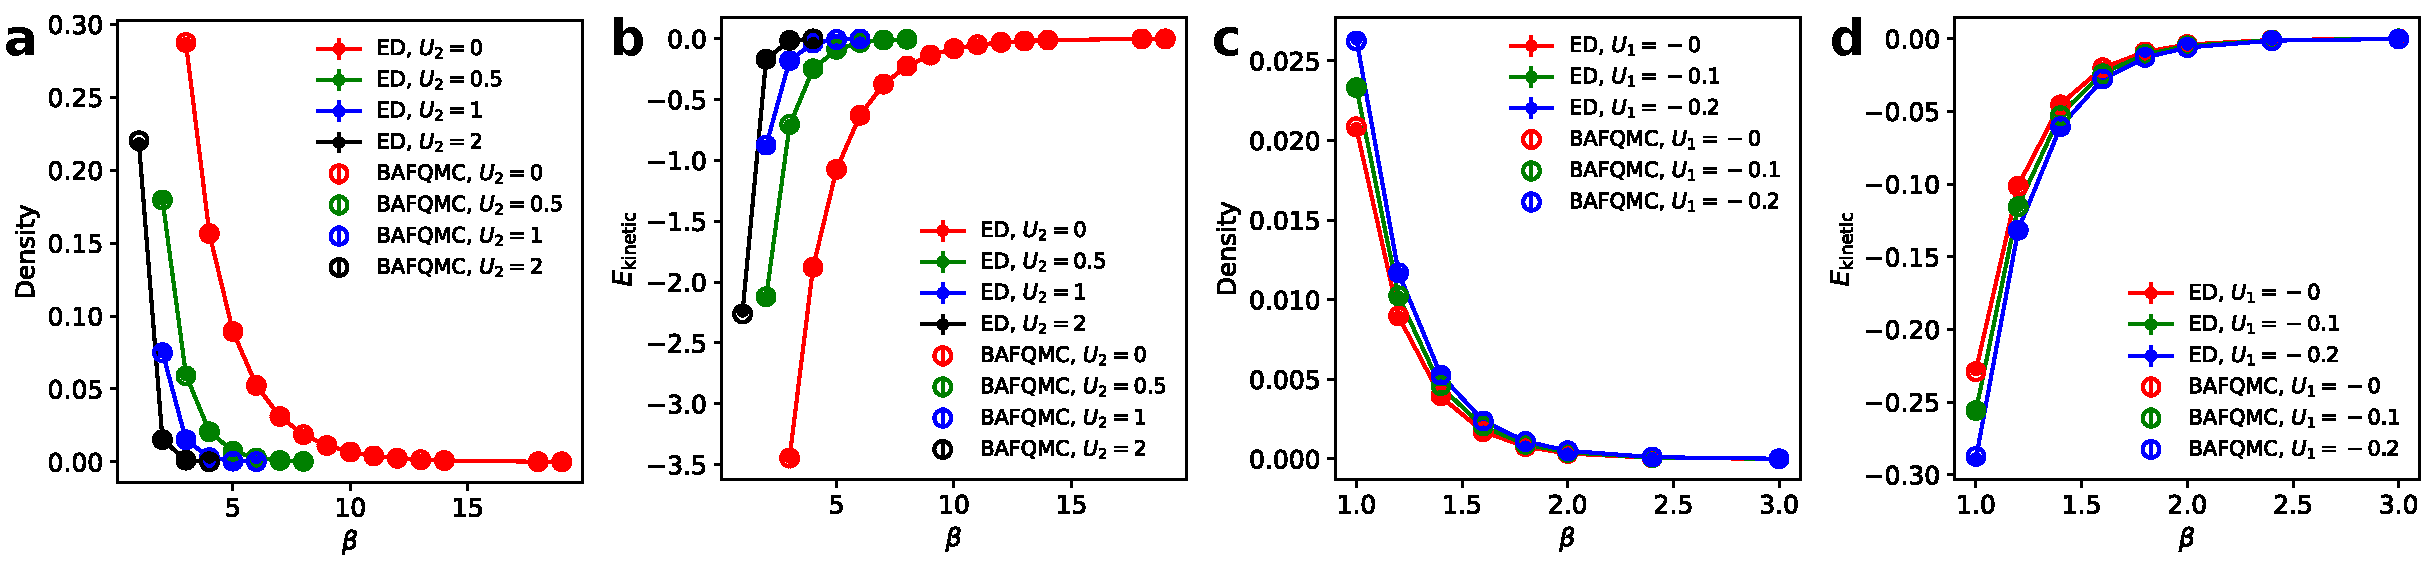
\includegraphics[width=\linewidth]{figures/benchmark.pdf}
    \caption{\textbf{Comparison of BPQMC calculation results and ED benchmark for the two-flavor frustrated Bose-Hubbard model at $2 \times 3$ sites.} (a)-(b), Variations of particle number density and kinetic energy with inverse temperature $\beta$ and interaction strength $U_2$, with fixed $\mu=-2.5$ for $U_1=0$. (c)-(d), Variations of particle number density and kinetic energy with inverse temperature $\beta$ and interaction strength $U_1$, with fixed $\mu=-5$ for $U_2=1$.}
    \label{fig:benchmark}
\end{figure*}

\section{Discussion}
\label{sec:discussion}

The central significance of this work is that it opens a new exact-simulation route for frustrated bosonic systems. Up to now, the standard sign-free domain for bosons and spins has been largely identified with models that are unfrustrated in a local basis. The present formulation shows that this boundary is not fundamental. Once the problem is rewritten in auxiliary-field language and the bosons are traced out analytically, the sign structure is controlled by symmetry properties of the HS-decoupled one-body propagators rather than by local matrix elements. This is why the upper-left quadrant of Fig.~\ref{fig:schematic}---frustrated systems with RP/TRS---becomes computable in BAFQMC. In that sense, the work is conceptually comparable to the role played by symmetry-protected determinantal QMC in fermionic systems: it enlarges the class of many-body problems that can be attacked exactly, and it does so in a way that is invisible from the usual world-line perspective.

At the same time, sign-problem-free does not mean numerically effortless. The bosonic determinant formulas carry a characteristic pole structure that has no direct analogue in fermionic AFQMC. In the number-conserving case, the sampling weight has the form $W(\phi)=\ee^{\sum_\ell \xi_\ell}\det(I_N-\mc B)^{-1}$, so poles appear whenever $1$ becomes an eigenvalue of the single-particle propagator $\mc B$. For sufficiently low chemical potential $\mu$, the boson density is dilute and the sampled configurations stay far from these poles; the algorithm is then well behaved. To access higher densities one must increase $\mu$, and the sampled distribution is pushed closer to the pole surface. Some configurations can then cross into sectors that look ``nonphysical'' if interpreted configuration by configuration: for example, the single-particle Green's function may suggest negative occupation numbers. Nevertheless, the normalized ensemble remains meaningful through the regularized, analytically continued interpretation of the weight discussed in Appendix~\ref{app:regularization}. In this sense, apparently nonphysical configurations are an unavoidable part of the regularized bosonic auxiliary-field ensemble, even though the final normalized observables remain physical.

The more serious difficulty is numerical rather than conceptual. When the interaction is strong, or when the temperature is lowered so that the imaginary-time evolution becomes longer, the weight distribution broadens and a nonnegligible fraction of configurations can approach the pole surface extremely closely. Their weights then become nearly divergent. This does not introduce a sign problem, but it can badly damage Monte Carlo stability and ergodicity and generate very large statistical errors. Lower temperature makes the problem worse because the product of many time slices produces a broader distribution of single-particle eigenvalues. In practice, this means that finite-temperature number-conserving BAFQMC is best suited to relatively dilute regimes, moderately high temperatures, and weak-to-intermediate interactions.

The paired case behaves differently and in an important sense more favorably. When anomalous terms are present, the boundary between physical and nonphysical configurations can be monitored through the smallest eigenvalue of the single-particle Green's function. For the sign-free paired models considered here, that boundary does not coincide with a pole of the sampling weight. As a consequence, one avoids the most severe numerical pathology of the number-conserving case, namely the appearance of almost divergent weights right at the edge of the physical region. This makes paired BAFQMC more stable in practice. The trade-off is that, in the paired finite-temperature models of this type, the particle number cannot be increased without bound by tuning the chemical potential. Instead, the accessible density remains capped, so the method is again most useful for relatively sparse bosonic systems rather than for very high-density regimes.

These observations delineate the practical regime of the present finite-temperature algorithm. The current BAFQMC framework is especially promising for dilute or moderately filled bosonic systems on frustrated lattices, at temperatures that are not too low and for interactions that are not too strong. This already covers a substantial and previously inaccessible class of problems. Looking ahead, a particularly important direction is the development of bosonic projector QMC schemes. A ground-state projector formulation may avoid the most damaging finite-temperature pole structure and could therefore extend sign-free BAFQMC deeper into low-temperature and stronger-coupling regimes. Establishing such a projector framework is, in our view, one of the most worthwhile next steps opened by the present work.

\section{Summary and outlook}
\label{sec:summary}







\bibliographystyle{apsrev4-2}
\bibliography{BAFQMC-draft}











\appendix

\section{Algebra of bosonic quadratic forms}
\label{app:algebra}

This appendix collects the algebraic identities underlying the BAFQMC formulas. Throughout, operator identities are first understood on the finite-particle subspace, which is invariant under polynomials in creation and annihilation operators. Whenever the relevant exponentials are well defined, the same identities extend by closure to their natural operator domains.

Consider the quadratic generator
\begin{equation}
    \hat h(A,\xi) = -\frac12\hat\chi^\trans\Omega A\hat\chi + \xi,
\end{equation}
with $A\in\mathfrak{sp}(2N,\mathbb C)$, i.e. $\Omega A+A^\trans\Omega=0$. The first step is to determine its action on the Nambu vector. Using $[XY,Z]=X[Y,Z]+[X,Z]Y$ together with $[\hat\chi_\mu,\hat\chi_\nu]=\Omega_{\mu\nu}$, one finds
\begin{equation}
\begin{aligned}
    [\hat h(A,\xi),\hat\chi_\lambda]
    ={}& -\frac12\sum_{\mu,\nu,\rho}
    \Omega_{\mu\nu}A_{\nu\rho}
    [\hat\chi_\mu\hat\chi_\rho,\hat\chi_\lambda] \\
    ={}& -\frac12\sum_{\mu,\nu,\rho}
    \Omega_{\mu\nu}A_{\nu\rho}
    \left(\hat\chi_\mu\Omega_{\rho\lambda}+\Omega_{\mu\lambda}\hat\chi_\rho\right).
\end{aligned}
\end{equation}
The first term is $-\frac12(\Omega A\Omega\hat\chi)_\lambda$, while the second is $+\frac12(A\hat\chi)_\lambda$. Using the symplectic condition in the form $\Omega A\Omega=A^\trans$, the two contributions combine to give
\begin{equation}
    [\hat h(A,\xi),\hat\chi] = -A\hat\chi.
    \label{eq:appendix_commutator}
\end{equation}
The corresponding exponential identities then follow from the Baker-Campbell-Hausdorff expansion:
\begin{equation}
    \ee^{\hat h(A,\xi)}\hat\chi\,\ee^{-\hat h(A,\xi)} = \ee^{-A}\hat\chi,
    \qquad
    \hat\chi\,\ee^{\hat h(A,\xi)} = \ee^{\hat h(A,\xi)}\ee^{A}\hat\chi.
\end{equation}
Iterating this relation over an ordered product immediately yields the transfer-matrix relation used in the main text,
\begin{equation}
    \hat\chi\,\prod_{\ell=1}^{L}\ee^{\hat h(A_\ell,\xi_\ell)}
    = \left(\prod_{\ell=1}^{L}\ee^{\hat h(A_\ell,\xi_\ell)}\right)
      \left(\prod_{\ell=1}^{L}\ee^{A_\ell}\right)\hat\chi,
\end{equation}
which is Eq.~\eqref{eq:Mdef}.

\section{Bosonic Gaussian trace formula}
\label{app:trace}

In this appendix we derive the trace formulas used in the main text. We first treat the number-conserving case by a direct coherent-state calculation and then explain the general paired formula and its branch structure.

\subsection{Number-conserving case}
\label{app:trace_number}

Consider a Gaussian operator of the form
\begin{equation}
    \hat U = \exp\left(\hat{\bb a}^{\hc} C\hat{\bb a} + \xi\right),
\end{equation}
where $C$ is an $N\times N$ matrix and $\xi$ is a scalar. Let $\|z\rangle = \exp(\hat{\bb a}^{\hc}z)|0\rangle$ denote the unnormalized bosonic coherent state, with $z\in\mathbb C^N$. The standard resolution of the identity is
\begin{equation}
    I = \int \frac{\dd^{2N}z}{\pi^N}\,\ee^{-z^\hc z}\,\|z\rangle\langle z\|,
\end{equation}
and the overlap is $\langle z\|w\rangle = \ee^{z^\hc w}$.

The operator $\hat U$ acts linearly on coherent states because
\begin{equation}
    \hat U\,\hat{\bb a}^{\hc}\hat U^{-1} = \hat{\bb a}^{\hc}\ee^C,
\end{equation}
which follows from $[\hat{\bb a}^{\hc}C\hat{\bb a},\hat a_i^\hc]=\sum_j \hat a_j^\hc C_{ji}$. Since the vacuum is annihilated by $\hat{\bb a}$ and is therefore invariant under $\hat U$, we obtain
\begin{equation}
    \hat U\|z\rangle = \ee^{\xi}\|\ee^C z\rangle.
\end{equation}
Consequently,
\begin{equation}
\begin{aligned}
    \Tr\,\hat U
    &= \int \frac{\dd^{2N}z}{\pi^N}\,\ee^{-z^\hc z}\langle z\|\hat U\|z\rangle \\
    &= \ee^{\xi}\int \frac{\dd^{2N}z}{\pi^N}\,\exp\left[-z^\hc(I_N-\ee^C)z\right].
\end{aligned}
\end{equation}
Whenever the Hermitian part of $I_N-\ee^C$ is positive, the Gaussian integral converges absolutely and evaluates to
\begin{equation}
    \Tr\,\hat U = \ee^{\xi}\det(I_N-\ee^C)^{-1}.
    \label{eq:number_trace_appendix}
\end{equation}
Because both sides are holomorphic in the entries of $\ee^C$ away from the pole $\det(I_N-\ee^C)=0$, the identity extends meromorphically to all matrices with $\det(I_N-\ee^C)\neq 0$. This proves Eq.~\eqref{eq:trace_formula_number} as an algebraic identity. In number-conserving BAFQMC, however, this meromorphic extension is not by itself the Monte Carlo interpretation when the auxiliary-field integral crosses the pole surface; Appendix~\ref{app:regularization} explains how the same determinant formula is then recovered from Gaussian-cutoff renormalization.

For an ordered product of number-conserving slices,
\begin{equation}
    \hat U = \prod_{\ell=1}^{L}\exp\left(\hat{\bb a}^{\hc}B_\ell\hat{\bb a}+\xi_\ell\right),
\end{equation}
the conjugation relation $\hat{\bb a}\,\hat U = \hat U\,\mc B\hat{\bb a}$ with $\mc B=\ee^{B_1}\cdots\ee^{B_L}$ implies that the product itself is represented by the same single-particle matrix $\mc B$. Hence
\begin{equation}
    \Tr\,\hat U = \exp\!\left(\sum_{\ell}\xi_\ell\right)\det(I_N-\mc B)^{-1},
\end{equation}
as stated in the main text.

\subsection{General paired case and branch choice}
\label{app:trace_paired}

For general Gaussian propagators with pairing terms, the trace is no longer given by an ordinary determinant but by a metaplectic character. Let
\begin{equation}
    \hat U = \prod_{\ell=1}^{L}\ee^{\hat h(A_\ell,\xi_\ell)},
    \qquad
    \mc M = \ee^{A_1}\cdots\ee^{A_L}.
\end{equation}
Whenever the trace converges and $\det(I_{2N}-\mc M)\neq 0$, the standard character formula for the metaplectic representation gives~\cite{thomas2008character}
\begin{equation}
    \Tr\,\hat U = \exp\!\left(\sum_{\ell}\xi_\ell\right)\det(I_{2N}-\mc M)^{-1/2},
    \label{eq:character_formula_appendix}
\end{equation}
where the square root must be interpreted on the metaplectic branch. We now explain how that branch is fixed.

The simplest reference region is the stable diagonal sector. Suppose that $\hat U$ is unitarily equivalent, via a bosonic Bogoliubov transformation, to a diagonal number-conserving Gaussian,
\begin{equation}
    \hat U \sim \exp\left(\sum_{j=1}^{N}\varepsilon_j\hat\beta_j^\hc\hat\beta_j + \xi\right),
    \qquad \Re\,\varepsilon_j < 0.
    \label{eq:stable_diagonal}
\end{equation}
Then
\begin{equation}
    \Tr\,\hat U = \ee^{\xi}\prod_{j=1}^{N}(1-\ee^{\varepsilon_j})^{-1}.
    \label{eq:diag_trace_paired}
\end{equation}
On the other hand, the associated Nambu transfer matrix is similar to
\begin{equation}
    \diag\left(\ee^{\varepsilon_1},\ldots,\ee^{\varepsilon_N},\ee^{-\varepsilon_1},\ldots,\ee^{-\varepsilon_N}\right).
\end{equation}
Hence $\det(I_{2N}-\mc M)$ is a perfect square up to the normal-ordering factor already absorbed into $\xi$, and Eq.~\eqref{eq:diag_trace_paired} fixes the relevant branch of the square root uniquely. In other words, the notation
\begin{equation}
    \det(I_{2N}-\mc M)^{-1/2}
\end{equation}
in the main text does \emph{not} mean the principal branch of the complex square root; it means the branch obtained by continuous continuation from the stable diagonal region, where the trace is unambiguously given by Eq.~\eqref{eq:diag_trace_paired}.

To extend the formula beyond that region, note that both sides of Eq.~\eqref{eq:character_formula_appendix} are holomorphic functions of the matrix entries of $\mc M$ on every connected component of the nonsingular manifold
\begin{equation}
    \{\mc M\in Sp(2N,\mathbb C)\; ;\; \det(I_{2N}-\mc M)\neq 0\}.
\end{equation}
Because they agree on the nonempty open subset corresponding to stable diagonal propagators, the identity theorem implies that they agree on the entire connected component. This yields Eq.~\eqref{eq:trace_formula_main}. Sign or phase ambiguities can only appear when a path in auxiliary-field space precisely crosses the pole $\det(I_{2N}-\mc M)=0$, exactly as expected from the metaplectic double cover.

\section{Equal-time Green's function and local-update ratio}
\label{app:green}

This appendix derives Eqs.~\eqref{eq:Gformula} and~\eqref{eq:update_ratio_main}.

\subsection{Equal-time Green's function}

Let
\begin{equation}
    \hat U = \prod_{\ell=1}^{L}\ee^{\hat h(A_\ell,\xi_\ell)},
    \qquad
    \mc M = \ee^{A_1}\cdots\ee^{A_L}.
\end{equation}
From Eq.~\eqref{eq:Mdef},
\begin{equation}
    \hat\chi\hat U = \hat U\mc M\hat\chi.
    \label{eq:chiUappendix}
\end{equation}
Multiply this identity on the right by $\hat\chi^\trans$ and take the trace:
\begin{equation}
    \Tr\left(\hat\chi\hat U\hat\chi^\trans\right)
    = \Tr\left(\hat U\mc M\hat\chi\hat\chi^\trans\right)
    = (\Tr\hat U)\,\mc M G,
    \label{eq:first_G_step}
\end{equation}
where $G$ is the matrix defined in Eq.~\eqref{eq:Gdef}. On the other hand, using $\hat\chi_\mu\hat\chi_\nu = \hat\chi_\nu\hat\chi_\mu + \Omega_{\mu\nu}$,
\begin{equation}
    \hat\chi\hat U\hat\chi^\trans = (\hat\chi\hat\chi^\trans-\Omega)\hat U,
\end{equation}
whence
\begin{equation}
    \Tr\left(\hat\chi\hat U\hat\chi^\trans\right)
    = (\Tr\hat U)(G-\Omega).
    \label{eq:second_G_step}
\end{equation}
Comparing Eqs.~\eqref{eq:first_G_step} and~\eqref{eq:second_G_step}, we find
\begin{equation}
    G-\Omega = \mc M G.
\end{equation}
Rearranging gives
\begin{equation}
    (I_{2N}-\mc M)G = \Omega,
\end{equation}
and therefore
\begin{equation}
    G = (I_{2N}-\mc M)^{-1}\Omega.
\end{equation}
This is Eq.~\eqref{eq:Gformula}.

\subsection{Update ratio}
\label{app:update}

Now suppose only slice $\ell$ changes, so that
\begin{equation}
    \ee^{A_\ell'} = (I_{2N}+\Delta_\ell)\ee^{A_\ell},
    \qquad
    \delta\xi_\ell = \xi_\ell'-\xi_\ell.
\end{equation}
Using the cyclic invariance of the trace, we are free to reorder the product so that slice $\ell$ appears first. Define
\begin{equation}
    \mc M_\ell = \ee^{A_\ell}\ee^{A_{\ell+1}}\cdots\ee^{A_L}\ee^{A_1}\cdots\ee^{A_{\ell-1}},
\end{equation}
and similarly
\begin{equation}
    \mc M_\ell' = (I_{2N}+\Delta_\ell)\mc M_\ell.
\end{equation}
Then
\begin{equation}
    \frac{W'}{W}
    = \ee^{\delta\xi_\ell}
      \frac{\det(I_{2N}-\mc M_\ell')^{-1/2}}{\det(I_{2N}-\mc M_\ell)^{-1/2}}.
\end{equation}
Factor the updated matrix as
\begin{equation}
\begin{aligned}
    I_{2N}-\mc M_\ell'
    &= I_{2N}-(I_{2N}+\Delta_\ell)\mc M_\ell \\
    &= \left[I_{2N}-\Delta_\ell(I_{2N}-\mc M_\ell)^{-1}\mc M_\ell\right]
       (I_{2N}-\mc M_\ell).
\end{aligned}
\end{equation}
Therefore
\begin{equation}
    \frac{W'}{W}
    = \ee^{\delta\xi_\ell}
      \det\left[I_{2N}-\Delta_\ell(I_{2N}-\mc M_\ell)^{-1}\mc M_\ell\right]^{-1/2}.
    \label{eq:update_intermediate}
\end{equation}
Using
\begin{equation}
    G_\ell\Omega^{-1} = (I_{2N}-\mc M_\ell)^{-1},
\end{equation}
and the identity
\begin{equation}
    I_{2N}-(I_{2N}-\mc M_\ell)^{-1} = -(I_{2N}-\mc M_\ell)^{-1}\mc M_\ell,
\end{equation}
Eq.~\eqref{eq:update_intermediate} becomes
\begin{equation}
    \frac{W'}{W}
    = \ee^{\delta\xi_\ell}
      \det\left[I_{2N}+\Delta_\ell\left(I_{2N}-G_\ell\Omega^{-1}\right)\right]^{-1/2},
\end{equation}
which is Eq.~\eqref{eq:update_ratio_main}.

\section{Regularized interpretation of the bosonic weight}
\label{app:regularization}

The bosonic Gaussian trace formula differs from the fermionic one in a crucial respect: the weight has poles. Specifically, due to the Pauli exclusion principle and fermionic statistics, the integrand of the Monte Carlo integral in fermionic AFQMC is proportional to
\begin{equation}
    W(\phi)\propto \det\left[I_N+\mc B(\phi)\right]\,.
\end{equation}
This is a holomorphic function, making the Monte Carlo sampling---which corresponds to the path integral over the auxiliary field $\phi$---directly well-defined. However, in BAFQMC, the integrand takes the form
\begin{equation}
    W(\phi)\propto\det\left[I_{2N}-\mc M(\phi)\right]^{-1/2}
    \;\text{or}\;
    \det\left[I_{N}-\mc B(\phi)\right]^{-1} \,.
\end{equation}
These expressions exhibit pole structures. In particular, in the number-conserving case, the path integral over the auxiliary field $\phi$ actually crosses the poles where $\det\left[I_{N}-\mc B(\phi)\right]=0$. Near these poles, the bare trace formula for the sampling weight intrinsically diverges, rendering its path integral ill-defined. Below, we provide a regularized interpretation of this situation, demonstrating that these divergent parts cancel exactly. Therefore, as long as the chemical potential $\mu$ is chosen within a physical (sufficiently low) range, the results obtained by sampling according to the standard BAFQMC procedure described in Sec.~\ref{sec:afqmc} remain exact and physical, even if a fraction of the sampled auxiliary-field configurations indeed cross the poles.

Let $r_1(\phi),\dots,r_N(\phi)$ be the eigenvalues of $\mc B(\phi)$. Formally, the bare bosonic trace is the generating series of all occupation-number sectors,
\begin{equation}
\begin{aligned}
    W_{\mathrm{bare}}(\phi)
    =& \exp\!\left[\sum_{\ell=1}^{L}\xi_\ell(\phi_\ell)\right]
    \sum_{n_1,\dots,n_N\ge0} a_{\bb n}(\phi), \\
    a_{\bb n}(\phi)={}& \prod_{i=1}^{N} r_i(\phi)^{n_i}.
\end{aligned}
\end{equation}
When $|r_i(\phi)|<1$ for all $i$, this series converges absolutely and reproduces Eq.~\eqref{eq:trace_formula_number}. If some eigenvalue moves outside the unit circle, however, large-occupation sectors are amplified rather than suppressed, and the bare trace ceases to exist. Physically this is why BAFQMC can encounter poles even though the final grand-canonical partition function is finite.

We therefore define, at fixed configuration $\phi$, the Gaussian-cutoff trace
\begin{equation}
\begin{aligned}
    W_{\Lambda}(\phi)
    ={}& \exp\!\left[\sum_{\ell=1}^{L}\xi_\ell(\phi_\ell)\right]
      \sum_{n_1,\dots,n_N\ge0} a_{\bb n}(\phi) \\
    &\times \exp\!\left[-\frac{|a_{\bb n}(\phi)|^2}{\Lambda^2}\right].
\end{aligned}
    \label{eq:gaussian_cutoff_weight}
\end{equation}
For every finite $\Lambda$, the extra Gaussian factor suppresses sufficiently large occupation sectors and the sum is absolutely convergent. The regulator is deliberately chosen in occupation-number space: it suppresses the bosonic states that are responsible for the divergence, rather than trying to move the configuration away from the pole by hand.

It is useful to see the mechanism first in one mode. If $W_{\mathrm{bare}}\sim \sum_{n\ge0} r^n$, then
\begin{equation}
    W_{\Lambda}(r)=\sum_{n\ge0} r^n \exp\!\left(-\frac{|r|^{2n}}{\Lambda^2}\right).
\end{equation}
For $|r|<1$, the regulator becomes irrelevant as $\Lambda\to\infty$ and $W_{\Lambda}(r)\to (1-r)^{-1}$. For $|r|>1$, the terms with $n\lesssim n_{*}(\Lambda)\equiv \ln\Lambda/\ln|r|$ are almost unsuppressed, so the regulated sum is well approximated by a large partial geometric series:
\begin{equation}
    W_{\Lambda}(r)\approx \sum_{n=0}^{n_{*}(\Lambda)} r^n
    = -\frac{r^{\,n_{*}(\Lambda)+1}}{1-r}+\frac{1}{1-r}.
\end{equation}
The first term is cutoff dependent and diverges with $\Lambda$; the second term is cutoff independent. The Gaussian cutoff therefore separates the regulated trace into a divergent piece and a finite piece. The multivariate series in Eq.~\eqref{eq:gaussian_cutoff_weight} behaves in the same way:
\begin{equation}
    W_{\Lambda}(\phi)
    = P_{\Lambda}(\phi)
    + W_{\mathrm{reg}}(\phi)
    + O(\Lambda^{-1}),
\end{equation}
where $P_{\Lambda}(\phi)$ collects all cutoff-dependent terms that vanish or diverge as $\Lambda\to\infty$, while the $\Lambda$-independent part is
\begin{equation}
\begin{aligned}
    W_{\mathrm{reg}}(\phi)
    ={}& \exp\!\left[\sum_{\ell=1}^{L}\xi_\ell(\phi_\ell)\right]
      \prod_{i=1}^{N}\frac{1}{1-r_i(\phi)} \\
    ={}& \exp\!\left[\sum_{\ell=1}^{L}\xi_\ell(\phi_\ell)\right]
      \det\!\left(I_N-\mc B(\phi)\right)^{-1}.
\end{aligned}
    \label{eq:reg_weight_appendix}
\end{equation}
This finite part coincides with the ordinary trace.

The full auxiliary-field partition function is therefore introduced in two steps. First one keeps the cutoff finite,
\begin{equation}
    Z_{\Lambda}
    = \int \mc D\phi\; P_{\mathrm{aux}}(\phi)\,W_{\Lambda}(\phi).
\end{equation}
Only after the auxiliary-field integral is performed does one remove the regulator:
\begin{equation}
    Z = \lim_{\Lambda\to\infty} Z_{\Lambda}.
\end{equation}
If the physical grand-canonical partition function is finite, the cutoff-dependent pieces contained in $P_{\Lambda}(\phi)$ must cancel after the full auxiliary-field integration; otherwise $Z_{\Lambda}$ would diverge. What survives is exactly the finite part in Eq.~\eqref{eq:reg_weight_appendix}, so that 
\begin{equation}
    Z
    = \int \mc D\phi\; P_{\mathrm{aux}}(\phi)\,W_{\mathrm{reg}}(\phi).
\end{equation}
This is why the determinant formula used in BAFQMC should be regarded, in the number-conserving pole-crossing problem, as a renormalized sampling weight rather than as a naive bare trace.


\section{Regularized reflection positivity from the semigroup viewpoint}
\label{app:regularized_rp}

This appendix rewrites the reflection-positivity criterion in the semigroup language~\cite{wei2024prb}. Its purpose is not to replace the cone proof of Sec.~\ref{sec:reflection}, which is the cleanest way to see positivity of the bare convergent trace. Rather, this appendix explains why the same positivity survives when the bosonic weight is understood through the regularized Gaussian formula used in BAFQMC.

We again work with two reflected sets of bosons, $\hat{\bb b}=(\hat b_1,\ldots,\hat b_M)^\trans$ and $\hat{\bb c}=(\hat c_1,\ldots,\hat c_M)^\trans$, and collect them into the Nambu spinor
\begin{equation}
    \hat\chi = (\hat{\bb b},\hat{\bb c},\hat{\bb b}^{\hc},\hat{\bb c}^{\hc})^\trans.
\end{equation}
A general quadratic generator is written as
\begin{equation}
    \hat h = -\frac12\hat\chi^\trans\Omega A\hat\chi,
\end{equation}
with $A\in\mathfrak{sp}(4M,\mathbb C)$. Making the reflected left/right structure explicit, one may parameterize $A$ as
\begin{equation}
    A=
    \begin{pmatrix}
        B_{11} & B_{12} & C_{11} & C_{12} \\
        B_{21} & B_{22} & C_{12}^\trans & C_{22} \\
        D_{11} & D_{12} & -B_{11}^\trans & -B_{21}^\trans \\
        D_{12}^\trans & D_{22} & -B_{12}^\trans & -B_{22}^\trans
    \end{pmatrix},
    \label{eq:A_reflected_general}
\end{equation}
where $C_{11}=C_{11}^\trans$, $C_{22}=C_{22}^\trans$, $D_{11}=D_{11}^\trans$, and $D_{22}=D_{22}^\trans$.

The reflection used in Sec.~\ref{sec:reflection} is represented on the single-particle space by $J_1$ followed by complex conjugation, with
\begin{equation}
    J_1=
    \begin{pmatrix}
        0 & I_M & 0 & 0 \\
        I_M & 0 & 0 & 0 \\
        0 & 0 & 0 & I_M \\
        0 & 0 & I_M & 0
    \end{pmatrix}.
\end{equation}
Reflection symmetry of the quadratic generator is therefore
\begin{equation}
    J_1^\trans A J_1 = \bar A.
    \label{eq:J1_reflection_condition}
\end{equation}
This is simply the matrix form of exchanging the $\hat b$ and $\hat c$ sectors while conjugating coefficients.

The semigroup viewpoint introduces a second anti-linear structure, represented by $J_2$ followed by complex conjugation,
\begin{equation}
    J_2=
    \begin{pmatrix}
        0 & I_M & 0 & 0 \\
        -I_M & 0 & 0 & 0 \\
        0 & 0 & 0 & I_M \\
        0 & 0 & -I_M & 0
    \end{pmatrix},
\end{equation}
and the associated Hermitian involution
\begin{equation}
    \eta = J_2\Omega,
    \qquad
    \eta^\hc = \eta,
    \qquad
    \eta^2 = I_{4M}.
\end{equation}
The role of $\eta$ is easy to state physically: it separates the part of the Gaussian evolution that merely preserves the natural indefinite metric from the part that produces genuine contraction or expansion. Matrices satisfying
\begin{equation}
    g^\hc\eta g = \eta
\end{equation}
form the maximal subgroup associated with this metric. Relaxing the equality to
\begin{equation}
    g^\hc\eta g - \eta \preceq 0
    \qquad\text{or}\qquad
    g^\hc\eta g - \eta \succeq 0
\end{equation}
defines the corresponding contraction and expansion semigroups.

With $J_2$ in hand, the reflected generator splits naturally into
\begin{equation}
    A = A_{+} + A_{-},
    \qquad
    A_{\pm} = \frac12\left(A \pm J_2^\trans \bar A J_2\right).
    \label{eq:Apm_def}
\end{equation}
This decomposition has a simple meaning. The $A_{+}$ part is even under the $J_2$ anti-linear symmetry and behaves like a metric-preserving piece. The $A_{-}$ part is odd under that symmetry and contains the couplings that control whether the evolution moves into a contraction or expansion sector.

Using Eqs.~\eqref{eq:A_reflected_general} and~\eqref{eq:Apm_def}, one finds
\begin{equation}
    A_{+}=
    \begin{pmatrix}
        B_{11} & 0 & C_{11} & 0 \\
        0 & \bar B_{11} & 0 & \bar C_{11} \\
        D_{11} & 0 & -\bar B_{11} & 0 \\
        0 & \bar D_{11} & 0 & -B_{11}
    \end{pmatrix},
    \label{eq:Aplus_form}
\end{equation}
where $C_{11}=C_{11}^\trans$ and $D_{11}=D_{11}^\trans$. Combining the symplectic condition with $J_2^\trans A_{+}J_2=\bar A_{+}$ gives
\begin{equation}
    A_{+}^\hc\eta + \eta A_{+} = 0.
\end{equation}
Therefore $\exp(A_{+})$ preserves the metric $\eta$. This is the part of the reflected Gaussian propagator that moves inside the maximal subgroup but does not change the sign structure of the regularized weight.

The complementary part is
\begin{equation}
    A_{-}=
    \begin{pmatrix}
        0 & B_{12} & 0 & C_{12} \\
        \bar B_{12} & 0 & \bar C_{12} & 0 \\
        0 & D_{12} & 0 & -B_{12}^{\hc} \\
        \bar D_{12} & 0 & -B_{12}^\trans & 0
    \end{pmatrix},
    \label{eq:Aminus_form}
\end{equation}
with $C_{12}=C_{12}^{\hc}$ and $D_{12}=D_{12}^{\hc}$. Unlike $A_{+}$, this piece is not metric-preserving. Instead, the combination $\eta A_{-}$ is Hermitian:
\begin{equation}
    \eta A_{-} = J_2\Omega A_{-} =
    \begin{pmatrix}
        \bar D_{12} & 0 & -B_{12}^\trans & 0 \\
        0 & -D_{12} & 0 & B_{12}^{\hc} \\
        -\bar B_{12} & 0 & -\bar C_{12} & 0 \\
        0 & B_{12} & 0 & C_{12}
    \end{pmatrix}.
    \label{eq:etaAminus}
\end{equation}
This makes the cone structure visible, but it becomes especially transparent after a simple reordering of basis. Introduce the permutation matrix
\begin{equation}
    \Pi=
    \begin{pmatrix}
        0 & 0 & 0 & I_M \\
        0 & I_M & 0 & 0 \\
        0 & 0 & I_M & 0 \\
        I_M & 0 & 0 & 0
    \end{pmatrix},
\end{equation}
which rearranges the block basis from $(\hat{\bb b},\hat{\bb c},\hat{\bb b}^{\hc},\hat{\bb c}^{\hc})$ to $(\hat{\bb c}^{\hc},\hat{\bb c},\hat{\bb b}^{\hc},\hat{\bb b})$. Then
\begin{equation}
    \Pi^\trans (\eta A_{-}) \Pi =
    \begin{pmatrix}
        K & 0 \\
        0 & -\bar K
    \end{pmatrix},
    \qquad
    K =
    \begin{pmatrix}
        C_{12} & B_{12} \\
        B_{12}^{\hc} & -D_{12}
    \end{pmatrix}.
    \label{eq:etaAminus_diag}
\end{equation}
So after this reordering, all the information in the cone part is reduced to a single Hermitian block $K$. This is the same object that appears in the operator formulation: positivity of the reflected bilinear couplings in Eq.~\eqref{eq:rp_block_form} is exactly the requirement
\begin{equation}
    K \succeq 0.
    \label{eq:K_positive}
\end{equation}
The semigroup meaning of Eq.~\eqref{eq:K_positive} is now immediate. One block in Eq.~\eqref{eq:etaAminus_diag} is positive, while the other is its negative complex conjugate. Equivalently, the reflected cone part always comes as a paired expansion sector together with its companion contraction sector. This is the single-particle version of reflection positivity.

Why does this help with the regularized bosonic weight? In the convergent region, positivity is already guaranteed by the cone argument of Sec.~\ref{sec:reflection}. For the paired RP sector we then move within a pole-free connected component and keep the same metaplectic branch. The point of the semigroup decomposition above is that it prevents the reflected Gaussian propagator from wandering arbitrarily in matrix space. The $A_{+}$ piece moves only inside the metric-preserving subgroup, while the $A_{-}$ piece enters through the paired block structure of Eq.~\eqref{eq:etaAminus_diag}. Starting from any convergent reflection-positive reference point, one can continuously deform the propagator within the same reflected semigroup sector without touching the singular locus, and the regularized determinant therefore stays on the same nonnegative branch. In this sense the semigroup structure is the single-particle image of RP for the paired regularized weight.

For an ordered product of reflection-positive slices, the same decomposition is applied slice by slice. The reflected structure is therefore preserved throughout the imaginary-time evolution, and the full BAFQMC configuration weight remains nonnegative after regularization as well. This statement is the paired counterpart of Appendix~\ref{app:regularization}: it relies on staying in one pole-free component rather than on subtracting cutoff-dependent divergences.

\section{Details of the time-reversal-symmetry argument}
\label{app:kramers}

We now spell out the time-reversal-symmetry argument used in Sec.~\ref{sec:trs}. The logic is the same as in the familiar Kramers pairing argument for antiunitary symmetries~\cite{sakurai2017modern}, except that here it is applied to the single-particle propagator $\mc B$, which need not be Hermitian. Let
\begin{equation}
    \mc B = \ee^{B_1}\cdots\ee^{B_L},
    \qquad
    U^\hc\overline{B_\ell}U = B_\ell,
    \qquad
    UU^*=-I_N.
\end{equation}
Since complex conjugation commutes with the matrix exponential,
\begin{equation}
    U^\hc\overline{\ee^{B_\ell}}U = \ee^{B_\ell},
\end{equation}
and hence, by multiplication,
\begin{equation}
    U^\hc\overline{\mc B}U = \mc B.
    \label{eq:Bsym_prod}
\end{equation}
Define the antiunitary operator $\Theta=UK$ on the single-particle space. Equation~\eqref{eq:Bsym_prod} is precisely the statement that $\Theta$ commutes with $\mc B$.

If $\mc Bv=\lambda v$, then
\begin{equation}
    \mc B(\Theta v)=\Theta(\mc Bv)=\lambda^*\Theta v,
\end{equation}
so nonreal eigenvalues appear in complex-conjugate pairs. The remaining issue is the multiplicity of real eigenvalues.

Let $r\in\mathbb R$ be a real eigenvalue, and let $\mc E_r$ be its generalized eigenspace,
\begin{equation}
    \mc E_r = \ker\left[(\mc B-rI_N)^m\right],
\end{equation}
for $m$ large enough that the kernel stabilizes. Because $\Theta$ commutes with $\mc B$, the space $\mc E_r$ is invariant under $\Theta$. Moreover, $\Theta^2=UU^*=-I_N$ on $\mc E_r$. We claim that this forces $\dim_\mathbb C \mc E_r$ to be even.

Indeed, if a nonzero vector $v\in\mc E_r$ satisfied $\Theta v = \alpha v$ for some complex $\alpha$, then applying $\Theta$ once more would give
\begin{equation}
    -v = \Theta^2 v = \Theta(\alpha v) = \overline{\alpha}\Theta v = |\alpha|^2 v,
\end{equation}
which is impossible. Thus $v$ and $\Theta v$ are linearly independent. Starting from any nonzero $v_1\in\mc E_r$, the pair $\{v_1,\Theta v_1\}$ spans a two-dimensional $\Theta$-invariant subspace. Repeating the construction on the orthogonal complement produces a basis of $\mc E_r$ in such pairs, so $\dim_\mathbb C\mc E_r$ is even. Since the dimension of $\mc E_r$ is exactly the algebraic multiplicity $m_r$ of the eigenvalue $r$, every real eigenvalue has even algebraic multiplicity.

We may therefore factor the characteristic polynomial of $\mc B$ as
\begin{equation}
    \det(xI_N-\mc B)
    = \prod_{\lambda\notin\mathbb R}(x-\lambda)(x-\lambda^*)
      \prod_{r\in\mathbb R}(x-r)^{m_r},
\end{equation}
with $m_r$ even. Setting $x=1$ yields
\begin{equation}
    \det(I_N-\mc B)
    = \prod_{\lambda\notin\mathbb R}|1-\lambda|^2
      \prod_{r\in\mathbb R}(1-r)^{m_r}
    \ge 0.
\end{equation}
Finally, since the slice scalars $\xi_\ell$ are real,
\begin{equation}
    W(\phi) = \exp\!\left(\sum_\ell \xi_\ell\right)\det(I_N-\mc B)^{-1}\ge 0,
\end{equation}
whenever the determinant is nonzero. This completes the time-reversal-symmetry argument.

\end{document}